\documentclass[12pt,letterpaper]{article}

%% Sectional units up to subsubsections are numbered. To number
%% subsections, but not subsubsections, decrease this counter to 2.
\setcounter{secnumdepth}{4}

%% Page layout (customized to letter paper and NYU requirements):
\setlength{\oddsidemargin}{-.25in}
\setlength{\textwidth}{7in}
\setlength{\topmargin}{.0in}
\setlength{\headheight}{0in}
\setlength{\headsep}{0in}
\setlength{\textheight}{8.5in}
\setlength{\footskip}{.5in}
%\setcounter{chapter}{1}
%\usepackage{layout} % defines the \layout command, see below

%% Controls spacing between lines (\doublespacing, \onehalfspacing, etc.):
\usepackage{setspace}
% Graphics:
\usepackage[final]{graphicx}
%\usepackage{graphicx} % use this line instead of the above to suppress graphics in draft copies
%\usepackage{graphpap} % \defines the \graphpaper command

% Indent first line of each section:
\usepackage{indentfirst}

% Good AMS stuff:
\usepackage{amsthm} % facilities for theorem-like environments
\usepackage[tbtags]{amsmath} % a lot of good stuff!
\usepackage{pgfplots}
% Fonts and symbols:
\usepackage{amsfonts}
\usepackage{amssymb}
%% Use the line below for official NYU version, which requires
%% double line spacing. For all other uses, this is unnecessary,
%% so the line can be commented out.
\doublespacing % requires package setspace, invoked above

%% Each of the following lines defines the \com command, which produces
%% a comment (notes for yourself, for instance) in the output file.
%% Example:    \com{this will appear as a comment in the output}
%% Choose (uncomment) only one of the three forms:
%\newcommand{\com}[1]{[/// {#1} ///]}       % between [/// and ///].
\newcommand{\com}[1]{\marginpar{\tiny #1}} % as (tiny) margin notes
\renewcommand{\le}{\leqslant}
\renewcommand{\ge}{\geqslant}
\renewcommand{\emptyset}{\ensuremath{\varnothing}}
\newcommand{\ds}{\displaystyle}
\newcommand{\R}{\ensuremath{\mathbb{R}}}
\newcommand{\Q}{\ensuremath{\mathbb{Q}}}
\newcommand{\Z}{\ensuremath{\mathbb{Z}}}
\newcommand{\N}{\ensuremath{\mathbb{N}}}
\newcommand{\T}{\ensuremath{\mathbb{T}}}
\newcommand{\eps}{\varepsilon}
\newcommand{\closure}[1]{\ensuremath{\overline{#1}}}
%\newcommand{\com}[1]{}                     % suppress all comments.

%% Cross-referencing utilities. Use one or the other--whichever you prefer--
%% but comment out both lines for final version.
%\usepackage{showlabels}
%\usepackage{showkeys}
\begin{document}
\pagenumbering{arabic}

\title{An easier KIFMM algorithm for\\axisymmetric surface density distributions}
\date{December 14, 2015}
\author{Victor Churchill}
\clearpage
\maketitle
\thispagestyle{empty}

\newpage

\section{Contribution of this project}

The original KIFMM paper by Ying, Biros, and Zorin, explored three data sets for the 3D case: densities distributed on the unit sphere, densities distributed uniformly on the unit cube, and densities distributed at the eight corners of the unit cube.

This project examines the case of a broader category of non-uniform distributions, surfaces of revolution that are rotationally symmetric with respect to the azimuthal angle, or axisymmetric, as in Figure 1. While the original 3D KIFMM may be able to handle densities distributed on surfaces of revolution, \cite{YBZ} explains that the implementation is difficult. This project proposes to work around this issue by employing the technique described in \cite{YYM} to replace the 3D integral equations required by the 3D KIFMM with their Fourier representations, sequences of 2D integral equations. In this way, we can avoid the 3D KIFMM in favor of repeatedly applying the 2D KIFMM to accelerate pairwise computations of densities distributed on an axisymmetric surfaces of revolution.

\section{Background}

\subsection{KIFMM}
The kernel-independent fast multipole method uses a continuous distribution of an equivalent density on a surface enclosing a box in the hierarchical tree to represent the potential generated by sources in that box, rather than using analytic multipole expansions as in the original FMM. This allows us to construct an efficient FMM that only requires kernel evaluations. The KIFMM is also relatively easy to implement, since in general it applies to an arbitrary kernel that is the fundamental solution of some elliptic PDE. To change the kernel in the original FMM, one would need to develop analytic multipole expansions for that kernel that may be difficult to produce.

The upward and downward formulation of the aforementioned equivalent densities and their translation are explained in detail in $\S3.2$ and shown in Figures 3, 4, 5, and 6.

\begin{figure}[!ht]
\begin{center}
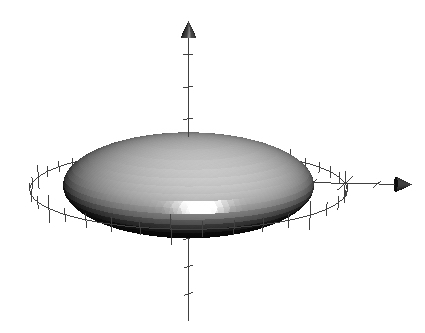
\includegraphics[scale=0.9]{/Users/HomeBase/Downloads/3dsurface}
\end{center}
\caption{An axisymmetric surface $\Gamma$ in 3D.}
\end{figure}

\subsection{Fourier representation of 3D integral equations}
Our strategy to apply the KIFMM to densities distributed on axisymmetric surfaces of revolution is grounded in the fact that it is easier to solve boundary integral equations defined on curves in $\mathbb{R}^2$ than those defined on surfaces in $\mathbb{R}^3$. This section is based on results in \cite{YYM}.

Consider the Fredholm integral equation of the first kind defined on the axisymmetric surface $\Gamma$ in 3D:
\begin{align}
\int_\Gamma k(\mathbf{x},\mathbf{y})\phi(\mathbf{y})d\mathbf{y} &= q(\mathbf{x}) &\mathbf{x}\in\Gamma
\end{align}
where $k$ is a kernel function, $\phi$ is an unknown density, and $q$ is a potential. This is exactly the same type of integral equation we see in the 3D KIFMM, in particular $(1)$ is the $S2M$ equation in \cite{YBZ}.

The surface $\Gamma$ is obtained by rotating a curve $\gamma$ about the $z$ axis. $\gamma$ is called the generating curve, shown in Figure 2. In particular, $\Gamma=\gamma\times\mathbb{T}$ where $\mathbb{T}$ is the one-dimensional torus (circle) parametrized by $\theta\in(-\pi,\pi]$. Since $k(\mathbf{x},\mathbf{y})$ is axisymmetric, we have that $k$ is a function only of the difference between $\theta$ and $\theta'$:
\begin{align}
k(\mathbf{x},\mathbf{y})=k(\theta-\theta',r,z,r',z')
\end{align}
where $\mathbf{x}=(r,z,\theta)$ and $\mathbf{y}=(r',z',\theta')$  in 3D cylindrical coordinates.

\begin{figure}[!ht]
\begin{center}
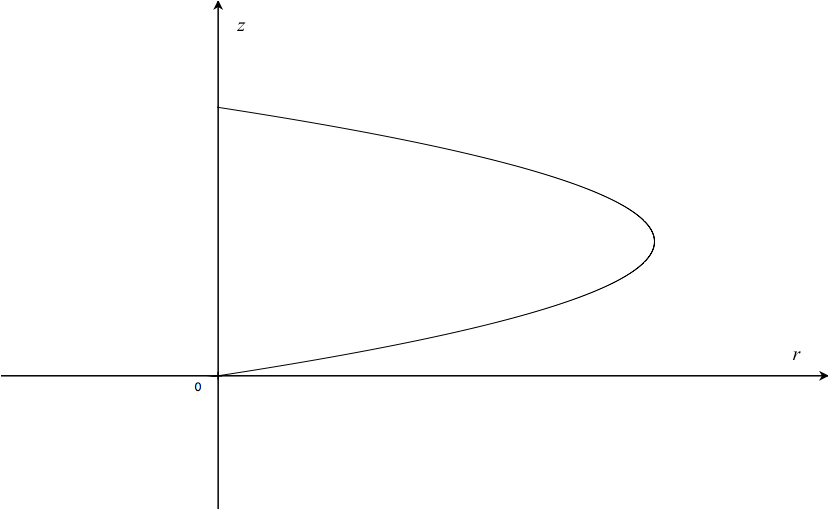
\includegraphics[scale=0.4]{/Users/HomeBase/Downloads/2dcurve}
\end{center}
\caption{The generating curve $\gamma$ in 2D, of an axisymmetric surface $\Gamma$ in 3D.}
\end{figure}

Due to these convenient circumstances, we can restate $(1)$ as a sequence of integral equations defined on the generating curve by performing a Fourier transform. If $\phi_n$, $q_n$, and $k_n$ are the Fourier modes of $k$, $\phi$, and $q$, then $(1)$ becomes:
\begin{align}
\sqrt{2\pi}\int_\gamma k_n(r,z,r',z')\phi_n(r',z')r'dl(r',z')&=q_n(r,z) &(r,z)\in\gamma, n\in\mathbb{Z}
\end{align}
where we have:
\begin{align}
q_n(r,z)&=\int_\mathbb{T}\frac{e^{-in\theta}}{\sqrt{2\pi}}q(r,z,\theta)d\theta&q(\mathbf{x})&=\sum_{n\in\mathbb{Z}}\frac{e^{in\theta}}{\sqrt{2\pi}}q_n(r,z)\\
\phi_n(r,z)&=\int_\mathbb{T}\frac{e^{-in\theta}}{\sqrt{2\pi}}\phi(r,z,\theta)d\theta&\phi(\mathbf{x})&=\sum_{n\in\mathbb{Z}}\frac{e^{in\theta}}{\sqrt{2\pi}}\phi_n(r,z)\\
k_n(r,z,r',z')&=\int_\mathbb{T}\frac{e^{-in\theta}}{\sqrt{2\pi}}k(r,z,r',z',\theta)d\theta&k(\mathbf{x},\mathbf{y})&=\sum_{n\in\mathbb{Z}}\frac{e^{in\theta}}{\sqrt{2\pi}}k_n(r,z,r',z')
\end{align}
In $\S3.2$, we'll apply this same transformation to the 3D integral equations prescribed in the 3D KIFMM, approximating with sequences of 2D integral equations that are easier to solve. For convenience, we can rewrite $(3)$ as:
\begin{align}
K_n\phi_n=q_n
\end{align}
If $K_n$ is a continuously invertible operator, we have:
%As in [2], we use Tikhonov regularization for a stable solve.
\begin{align}
\phi_n=K_n^{-1}q_n
%\phi_n=[\alpha I+K_n^TK_n]K_n^Tq_n
\end{align}
When we implement this strategy in combination with the KIFMM, we'll use Tikhonov regularization to stably solve $(8)$. Plugging in to $(6)$ gives the solution of the original 3D surface integral equation $(1)$:
\begin{align}
\phi(r,z,\theta)=\sum_{n\in\mathbb{Z}}\frac{e^{in\theta}}{\sqrt{2\pi}}[K_n^{-1}q_n](r,z)
%\phi(r,z,\theta)=\sum_{n\in\mathbb{Z}}\frac{e^{in\theta}}{\sqrt{2\pi}}\big[(\alpha I + K_n^TK_n)^{-1}K_n^Tq_n\big](r,z)
\end{align}
In practice, we choose a truncation parameter, $N$, such that $||q-\sum\limits_{n=-N}^{N}\frac{e^{in\theta}}{\sqrt{2\pi}}q_n||\le\epsilon$:
\begin{align}
\phi_{approx}=\sum_{n=-N}^N\frac{e^{in\theta}}{\sqrt{2\pi}}K_n^{-1}q_n
\end{align}

\section{Application of the KIFMM}
In this section we use the Fourier representation of surface integral equations described in $\S2.2$ together with the 2D KIFMM to create a fast algorithm for densities distributed on axisymmetric surfaces of revolution. Notation in this section for the surfaces follows \cite{YBZ}.

\subsection{Single-layer 3D Laplace kernel}
For now, we apply the algorithm considering only the single-layer 3D Laplace kernel. This choice has been made because its Fourier modes can be solved for analytically. For many other kernels, that is not that case, and we would need to approximate the modes using a discretization. This is left for future work.

We find the Fourier modes for this kernel below as in \cite{YYM}. For $\mathbf{x}=(r,z,\theta)$ and $\mathbf{y}=(r',z',\theta')$:
\begin{align}
k(\mathbf{x},\mathbf{y})&=\frac{1}{4\pi |\mathbf{x}-\mathbf{y}|}\\
&=\frac{1}{4\pi\sqrt{r^2+r'^2-2rr'\cos{(\theta-\theta')}+(z-z')^2}}\\
&=\sum_{n\in\mathbb{Z}}\frac{e^{in\theta}}{\sqrt{2\pi}}k_n(r,z,r',z')\\
\mbox{where }k_n(r,z,r',z')&=\frac{1}{\sqrt{8\pi^3rr'}}Q_{n-\frac{1}{2}}\bigg(\frac{r^2+(r')^2+(z-z')^2}{2rr'}\bigg)
\end{align}
and $Q_{n-\frac{1}{2}}$ is the half-integer order Legendre function of the second kind.

Notice that $k_n$ does not depend only on the difference between each coordinate, e.g. $(r-r')$. This has implications for the translation operators we construct for the KIFMM which is discussed in $\S3.2.4$.

\subsection{Full algorithm}
Recall that in the 3D KIFMM, we needed to solve surface integral equations like:
\begin{align}
\mbox{S2M: }&\int_{\mathbf{y}^{B,u}}{k(\mathbf{x},\mathbf{y})}\phi^{B,u}{(\mathbf{y})}d\mathbf{y}=\sum\limits_{i\in I_s^B} k(\mathbf{x},\mathbf{y}_i)\phi_i\mbox{ for all }\mathbf{x}\in\mathbf{x}^{B,u}
\end{align}
We can write $(15)$ as a sequence of 2D equations, $(16)$, by using the Fourier representation explained in $\S2.2$. If this is unclear, equation $(15)$ is to $(16)$ as equation $(1)$ is to $(3)$. In calculations below, I will skip this derivation and just state the sequences of 2D equations.

Now that we have our kernel $k_n$, we proceed through the standard 2D KIFMM algorithm for the sources on the 2D generating curve $\gamma$ \textbf{for each} $n\in[-N,-N+1,\dots,N]$ where $N$ is the truncation parameter chosen earlier in $(10)$. The KIFMM algorithm is very similar to the FMM algorithm described in \cite{CGR}, apart from how the equivalent densities are represented, and how the translation operators are computed. As mentioned earlier, rather than by multipole expansions, the potential due to sources in a box is matched to an equivalent density at discretization points on a surface enclosing the box. In 2D, these surfaces are circles with radii prescribed in \cite{YBZ}. To compute these equivalent densities, we will need to discretize several integral operators on different surfaces, which is explained in $\S3.2.2$.

In the following equations, $\mathbf{x}=(r,z)$ and $\mathbf{y}=(r',z')$. Also, please note the seemingly out-of-place $r'$ term under each integral, and recall that this is actually part of the integral operator $K_n$ as in $(3)$.
\subsubsection{Equivalent densities}
After partitioning the hierarchical tree with no more than a prescribed number of sources in each box, compute the upward equivalent density for each leaf box. Similar to the \textbf{S2M} step in the FMM, solving the following equation for $\phi^{B,u}$ gives the upward equivalent density for a box $B$ in the KIFMM:
\begin{align}
\mbox{S2M: }&\int_{\mathbf{y}^{B,u}}{k_n(\mathbf{x},\mathbf{y})}\phi^{B,u}_n{(\mathbf{y})}r'd\mathbf{y}=\sum\limits_{i\in I_s^B} k_n(\mathbf{x},\mathbf{y}_i)\phi_ir'_i\mbox{ for all }\mathbf{x}\in\mathbf{x}^{B,u}\\
\mbox{Discretized S2M: }&M_n\phi^{B,u}_n=q_n^{B,u}
\end{align}
where in $(17)$, $M_n$ is the matrix of kernel evaluations of pairs of discretization points on the upward check surface and upward equivalent surface of a box $B$, $q_n^{B,u}$ is the upward check potential, and the densities at the actual source points in the box are $\phi_i$. This is similar to $(7)$, and this process is illustrated in Figure 3. Once the upward equivalent density is computed for each leaf box, we use translation operators to find the upward and downward equivalent densities for every other box.

\begin{figure}[!ht]
\begin{center}
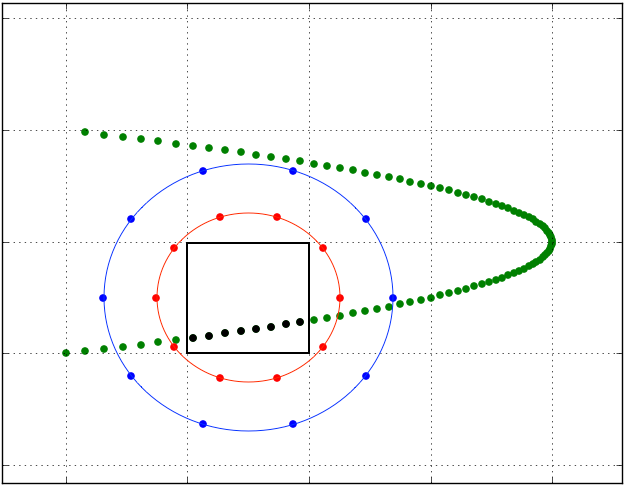
\includegraphics[scale=0.5]{/Users/HomeBase/Downloads/ued-curve}
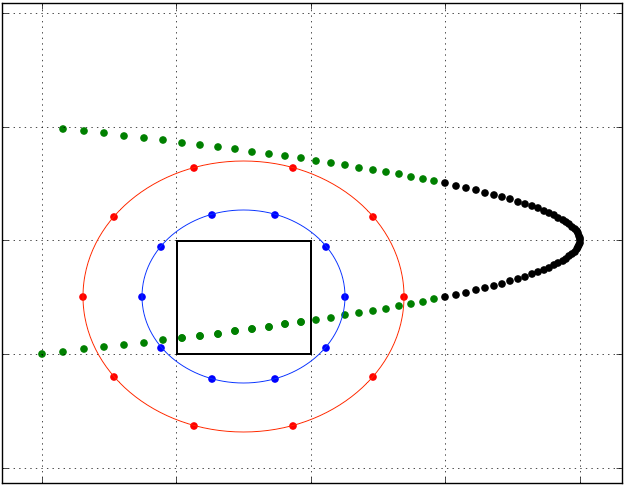
\includegraphics[scale=0.5]{/Users/HomeBase/Downloads/ded-curve}
\end{center}
\caption{Left: The upward check (blue) and equivalent (red) surfaces of a box used to compute the upward equivalent density due to source densities (black) in the box. Right: The downward check (blue) and equivalent (red) surfaces of a box used to compute the downward equivalent density due to sources densities (black) in the far field on the box. In the algorithm, we never actually directly compute a downward equivalent density.}
\end{figure}

\subsubsection{Translation Operators}

Translation operators limit the number of equivalent densities we need to compute directly by translating upward equivalent densities of the leaf boxes to upward and downward equivalent densities of all other boxes. In the KIFMM in particular, the translation operators in their discretized form are matrices that translate an equivalent density from one box to that of another. They are a pre-computation, as they are constant regardless of the source distribution.

In the previous step, we computed the upward equivalent density for each leaf box. The \textbf{M2M} operator translates the upward equivalent density from a leaf box $A$ to the upward equivalent density of its parent box $B$. Solving the following equation for $\phi_n^{B,u}$ gives the M2M operator.
\begin{align}
\mbox{M2M: }&\int_{\mathbf{y}^{B,u}}{k_n(\mathbf{x},\mathbf{y})}\phi^{B,u}_n{(\mathbf{y})}r'd\mathbf{y} = \int_{\mathbf{y}^{A,u}}{k_n(\mathbf{x},\mathbf{y})}\phi^{A,u}_n{(\mathbf{y})}r'd\mathbf{y}\mbox{ for all }\mathbf{x}\in\mathbf{x}^{B,u}\\
\mbox{Discretized M2M: }&M_n^B\phi^{B,u}_n=M_n^A\phi^{A,u}_n
\end{align}
where $M_n^A$ is the matrix of kernel evaluations of pairs of discretization points on the upward check surface of box $B$ and the upward equivalent surface of box $A$, and $M_n^B$ is the matrix of kernel evaluations of pairs of discretization points on the upward check surface of box $B$ and the upward equivalent surface of box $B$. Figure 4 gives a graphical representation of this step.
\begin{figure}[!ht]
\begin{center}
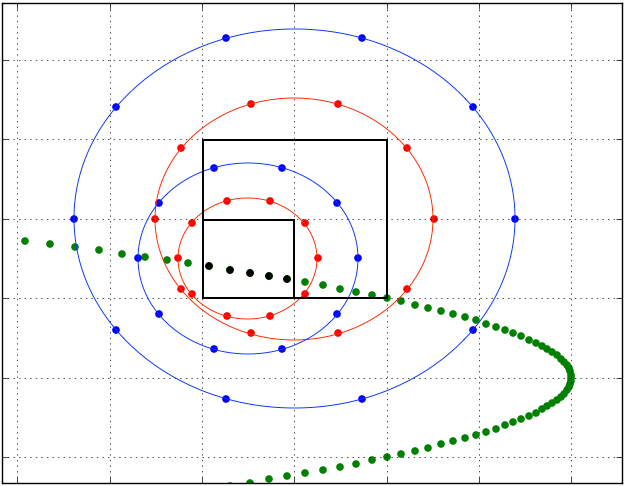
\includegraphics[scale=0.5]{/Users/HomeBase/Downloads/M2M-curve}
\end{center}
\caption{The upward equivalent density due to the source densities (black) in the child box computed from the upward equivalent (red) and check (blue) surfaces of the child box is translated to the upward equivalent density of the parent box, checking against its upward check (blue) and equivalent (red) surfaces.}
\end{figure}

After repeating that step, every box now has an upward equivalent density. The \textbf{M2L} operator translates the upward equivalent density from a non-leaf box $A$ to the downward equivalent density of a box $B$ on the same level.
\begin{align}
\mbox{M2L: }&\int_{\mathbf{y}^{B,d}}{k_n(\mathbf{x},\mathbf{y})}\phi^{B,d}_n{(\mathbf{y})}r'd\mathbf{y} = \int_{\mathbf{y}^{A,u}}{k_n(\mathbf{x},\mathbf{y})}\phi^{A,u}_n{(\mathbf{y})}r'd\mathbf{y}\mbox{ for all }\mathbf{x}\in\mathbf{x}^{B,d}\\
\mbox{Discretized M2L: }&M_n^B\phi^{B,d}_n=M_n^A\phi^{A,u}_n
\end{align}
where $M_n^A$ is the matrix of kernel evaluations of pairs of discretization points on the downward check surface of box $B$ and the upward equivalent surface of box $A$, and $M_n^B$ is the matrix of kernel evaluations of pairs of discretization points on the downward check surface of box $B$ and the downward equivalent surface of box $B$.

\begin{figure}[!ht]
\begin{center}
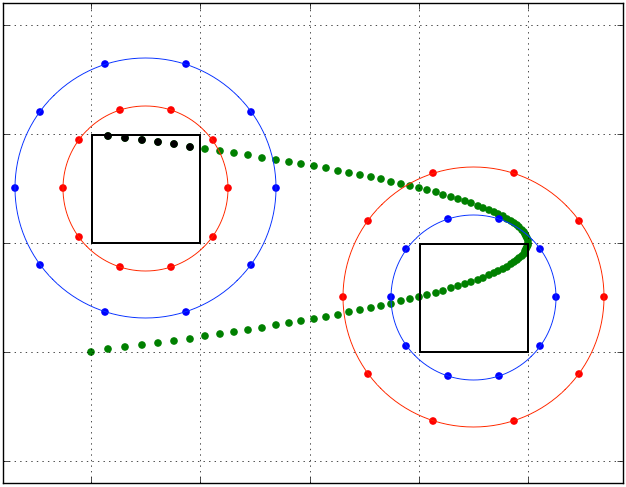
\includegraphics[scale=0.5]{/Users/HomeBase/Downloads/M2L-curve}
\end{center}
\caption{The upward equivalent density due to the source densities (black) in a box computed from the upward equivalent (red) and check (blue) surfaces of the child box is translated to the downward equivalent density of another box on the same level, checking against its upward check (blue) and equivalent (red) surfaces.}
\end{figure}

After repeating that step, every non-leaf box has a downward equivalent density. The \textbf{L2L} operator translates the downward equivalent density of a non-leaf box $A$ to the downward equivalent density of a child box $B$.
\begin{align}
\mbox{L2L: }&\int_{\mathbf{y}^{B,d}}{k_n(\mathbf{x},\mathbf{y})}\phi^{B,d}_n{(\mathbf{y})}r'd\mathbf{y}=\int_{\mathbf{y}^{A,d}}{k_n(\mathbf{x},\mathbf{y})}\phi^{A,d}_n{(\mathbf{y})}r'd\mathbf{y}\mbox{ for all }\mathbf{x}\in\mathbf{x}^{B,d}\\
\mbox{Discretized L2L: }&M_n^B\phi^{B,d}_n=M_n^A\phi^{A,d}_n
\end{align}
where $M_n^A$ is the matrix of kernel evaluations of pairs of discretization points on the downward check surface of box $B$ and the downward equivalent surface of box $A$, and $M_n^B$ is the matrix of kernel evaluations of pairs of discretization points on the downward check surface of box $B$ and the downward equivalent surface of box $B$. After repeating this step, every box now has an upward and downward equivalent density.

\begin{figure}[!ht]
\begin{center}
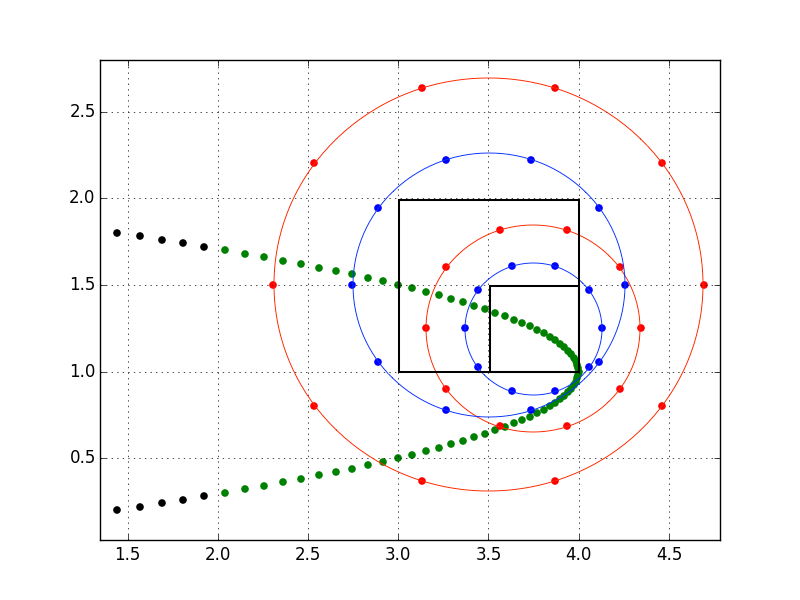
\includegraphics[scale=0.5]{/Users/HomeBase/Downloads/L2L-curve}
\end{center}
\caption{The downward equivalent density due to the source densities (black) in a parent box computed from the upward equivalent (red) and check (blue) surfaces of the parent box is translated to the downward equivalent density of a child box, checking against its upward check (blue) and equivalent (red) surfaces.}
\end{figure}

Once we have these upward and downward equivalent densities for every $n\in[-N,\dots,N]$, then we can reconstruct the 3D equivalent densities $\phi_{approx}$ by summing as in $(10)$. This summing can be accelerated via the FFT. Having these equivalent densities in 3D, we can complete the last step of the KIFMM algorithm by evaluating the far- and then near-field interactions.

Note that all requirements for smoothness and uniqueness of the solution to the integral equations in the KIFMM listed in $\S3.1.5$ of \cite{YBZ} (mostly pertaining to the sizes and positions of the surfaces) are satisfied here.

\subsubsection{Discretization details}
The equations in $\S3.2.1$ are discretized using $p$ points on the equivalent and check surfaces. $p$ is constant for all boxes, and the choice of $p$ determines the error level of the computations.This discretization requires two steps. First, the right hand side is the evaluation of a check potential. This step checks that the potential represented by the equivalent density and the actual source densities are the same to all boxes in the far field. Then on the left hand side, we invert a Dirichlet-type boundary integral equation to obtain the equivalent density. To stably solve this equation, as in \cite{YBZ}, we use Tikhonov regularization with regularization parameter $\alpha=10^{-12}$. Essentially, each translation is simply applying a series of matrices.

For example, the M2L operator is the matrix $T^{M2L}_n$ for a mode $n$ is obtained by solving $(20)$:
\begin{align}
\phi^{B,d}_n&=\bigg[\big[\alpha I +(K_n^B)^TK_n^B\big](K_n^B)^TK_n^A\bigg]\phi^{A,u}_n\\
\implies T^{M2L}_n &= \bigg[\big[\alpha I +(K_n^B)^TK_n^B\big](K_n^B)^TK_n^A\bigg]
\end{align}

\subsubsection{Non-uniform translation operators}
It's important to note that in the original KIFMM, translation operators only differ based on relative position and level in the hierarchical tree. This is because the kernels used there only depended the relative difference between coordinate values, e.g. $(r-r')$. As mentioned in $\S3.1$, for the single-layer Laplace kernel, however, we are not so lucky and so we need to look for some other relationship between the translation operators.

In particular, we notice from $(3)$ and $(14)$ that each integral operator 
\begin{align}
K_n = k_n(r,z,r',z')r'=\sqrt{\frac{r'}{8\pi^3r}}Q_{n-\frac{1}{2}}\bigg(\frac{r^2+(r')^2+(z-z')^2}{2rr'}\bigg)
\end{align}
depends on $\frac{r^2+(r')^2+(z-z')^2}{2rr'}$ and a constant $\sqrt{\frac{r'}{8\pi^3r}}$. Consequently, the translation operators depend on these same values.

For example, take $\frac{r^2+(r')^2+(z-z')^2}{2rr'}$ and $\sqrt{\frac{r'}{8\pi^3r}}$ as the arguments in consideration for an M2L operator from one box to a box horizontally one unit away. If we wanted to know the M2L operator from that same box to a box horizontally two units away, we could substitute $r'+1$ for $r'$ and see that now the operator depends on $\frac{r^2+(r')^2+2r'+1+(z-z')^2}{2rr'+2r}$ and $\sqrt{\frac{r'}{8\pi^3r}+\frac{1}{8\pi^3r}}$. 

One relationship we have noticed is that M2M operators, holding their global and relative positions constant, were the same regardless of the size of the box. That is, if you had child, parent, and grandparent boxes such that the bottom left corner was the same for every box, the child was the bottom left quadrant of the parent, and the parent was the bottom left quadrant of the grandparent, then the M2M operator from the child to the parent was the same as from the parent to the grandparent. We suspect this may be the same for L2L as well.

In future work, we hope to find concrete relationships between the translation operators to minimize the pre-computation. Otherwise we'd have to compute every translation operator in the entire computational domain which would be expensive.

\section{Implementation and Future Work}
Currently, we are able to produce all equivalent densities and translation operators with programs written and tested in Python, using the single-layer 3D Laplace kernel's Fourier modes. We have tested with several non-circular axisymmetric surfaces of revolution.

Much of the future work to do is in fully implementing the algorithm in Python. One key piece of this will be accelerating the matrix operations in $\S3$ using singular value decomposition (SVD) and other acceleration techniques described in \cite{MV}. SVD is applicable in this scenario since all interactions in the far field are low rank for many kernels.

In addition, in $\S3.1$ we mentioned that this strategy is currently only applicable to the single-layer Laplace kernel because of the convenient analytic determination of its Fourier modes. We hope to be able to apply this strategy to other kernels as well by discretizing them as in \cite{YYM}.

Other implementation work that needs to be done is testing various kernels, surfaces, and potentials, to perhaps find a methodical way to determine the optimal number of discretization points $p$ and the truncation parameter $N$.

Lastly, once the algorithm is completely accelerated and applicable to different kernels, performing error and computational analysis will be an important part of its evaluation as a fast method.

\begin{thebibliography}{99}\addcontentsline{toc}{chapter}{Bibliography}

\bibitem{CGR} Cheng, H., Greengard, L., Rokhlin, V., \emph{A Fast Adaptive Multipole Algorithm in Three Dimensions}. Journal of Computational Physics, 155, (1999), 468-498.

%\bibitem{HMY} Hao, S., Martinsson, P.G., Young, P., \emph{An efficient and highly accurate solver for multi-body acoustic scattering problems involving rotationally symmetric scatterers}. Computers and Mathematics with Applications, 69, (2015), 304-318.

\bibitem{MV} Martinsson, P.G., Rokhlin, V., \emph{An accelerated kernel-independent fast multipole method in one dimension}. SIAM Journal of Scientific Computing, Vol. 29, No. 3, (2007), 1160-1178.

\bibitem{YBZ} Ying, L., Biros, G., Zorin, D., \emph{A kernel-independent adaptive fast multipole method algorithm in two and three dimensions}. Journal of Computational Physics, 196, (2004), 591-626.

\bibitem{YYM} Young, P., Yao, S., Martinsson, P.G., \emph{A high-order Nystr{\"o}m discretization scheme for boundary integral equations defined on rotationally symmetric surfaces}. Journal of Computational Physics, 231, (2012), 4142-4159.

\end{thebibliography}

\end{document}
